% ============================================================
%  example.tex — демонстрационный документ для конвертации в docx
%  Сборка PDF:   pdflatex example && bibtex example && pdflatex example && pdflatex example
%  Конвертация:  см. convert.sh  /  README.md
% ============================================================
\documentclass[12pt, a4paper]{article}
%
% --- Кодировки и язык ---
\usepackage[T2A]{fontenc}
\usepackage[utf8]{inputenc}
\usepackage[english, russian]{babel}
\usepackage{cmap}

% --- Математика ---
\usepackage{amsmath, amssymb}

% --- Физические величины ---
%\usepackage[exponent-product = \cdot, output-decimal-marker = {,}]{siunitx}
%\input{siunitx-local-units}
\usepackage[version=4]{mhchem}

% --- Рисунки ---
\usepackage{graphicx}

% --- Библиография ---
\usepackage[backend=biber, style=gost-numeric, natbib=true]{biblatex}
\addbibresource{main.bib}

% --- Гиперссылки и перекрёстные ссылки ---
\usepackage[colorlinks=true, linkcolor=blue, citecolor=blue]{hyperref}
\usepackage{cleveref}     % Обычно загружается последним


\DeclareUnicodeCharacter{21CC}{\ensuremath{\rightleftharpoons}}


% ============================================================
%  Метаданные документа
% ============================================================
\title{Модель начального этапа окисление железа в жидком свинце}
\author{Даниил Колотинский\thanks{ОИВТ РАН,
        \texttt{kolotinskiy.da@phystech.edu}}}
\date{\today}

% ============================================================
\begin{document}
% ============================================================

\maketitle

\begin{abstract}

\end{abstract}

\tableofcontents
\newpage

% ============================================================
\section{Теория}
\label{sec:intro}

Рассматривается одномерная нестационарная задача начального окисления железа в жидком свинце вблизи поверхности стали. Координата $z$ отсчитывается по нормали к поверхности стали, причём $z=0$ соответствует межфазной границе ``сталь--свинец'', а $z=l$ --- внешней границе диффузионного слоя в жидком металле. Предполагается, что в пределах слоя толщины $l$ эволюция системы определяется только диффузией растворённого кислорода и растворённого железа, а конвективный перенос учитывается неявно через задание конечной толщины диффузионного слоя и граничных условий на его внешней границе. Схема рассматриваемой системы приведена на  рис.~\ref{fig:scheme}.

\begin{figure}[h!]
\centering
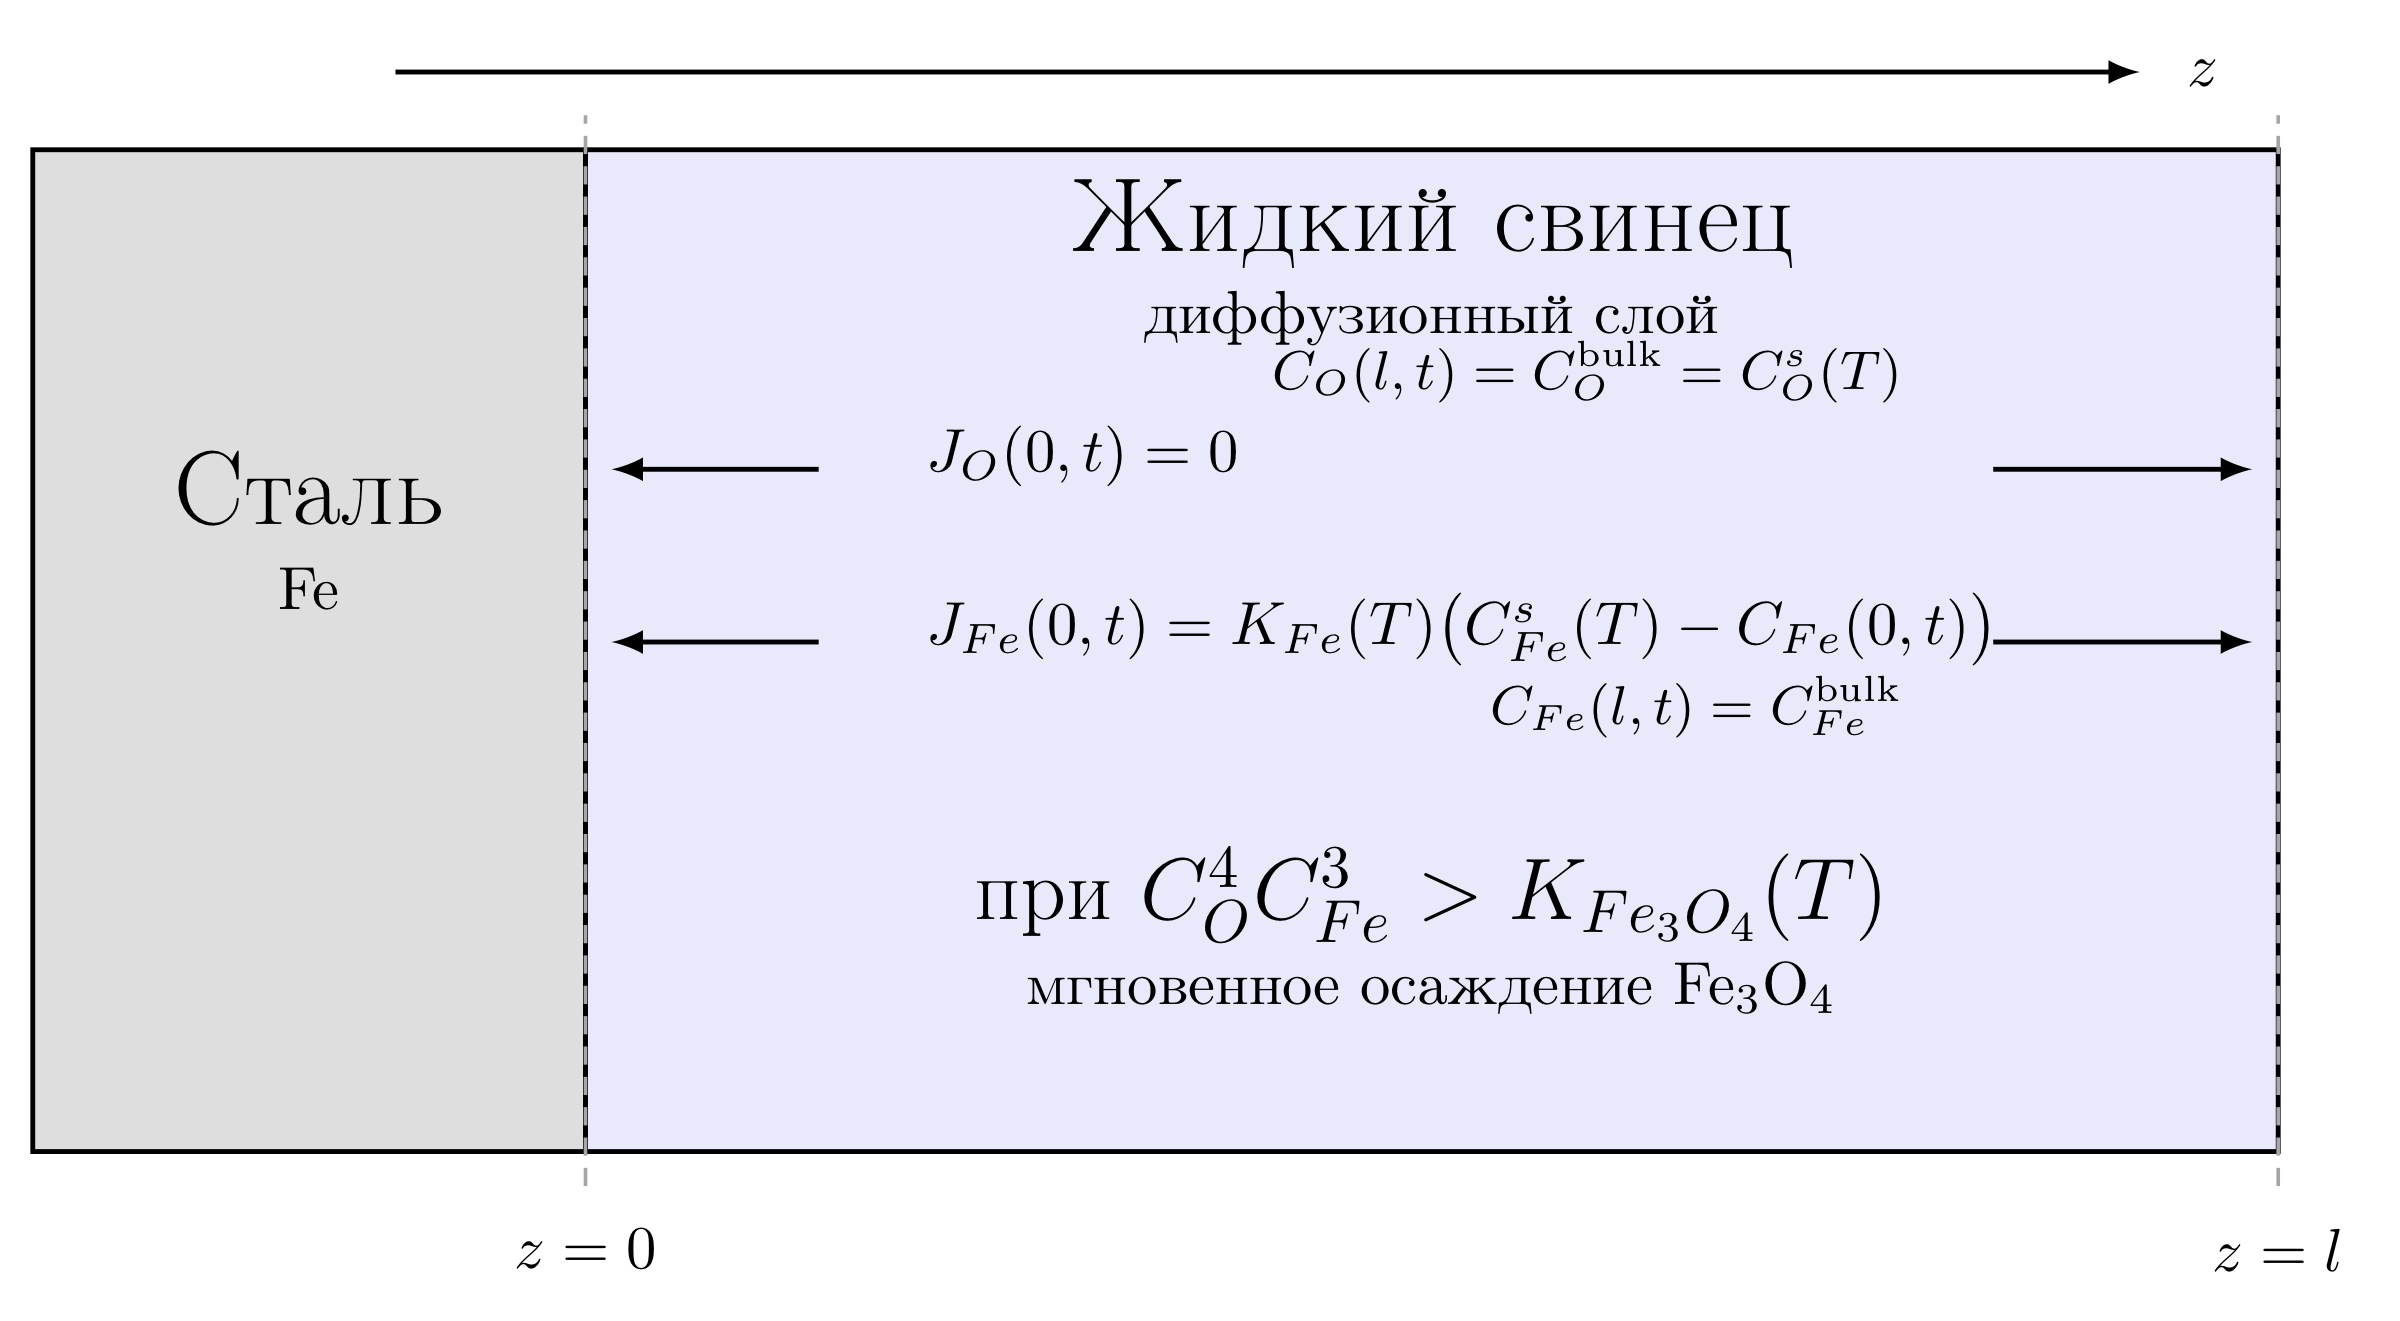
\includegraphics[width=\textwidth]{diagram.png}
\caption{Схема рассматриваемой системы и используемых граничных условий.}
\label{fig:scheme}
\end{figure}

\subsection*{Основные допущения}

При построении модели принимаются следующие допущения.
\begin{enumerate}
    \item Задача является одномерной: все искомые величины зависят только от координаты $z$ и времени $t$.
    \item Температура $T$ постоянна во всём объёме системы, поэтому все термодинамические и кинетические коэффициенты являются функциями только температуры.
    \item В жидком свинце рассматриваются только два растворённых компонента: кислород с концентрацией $C_O(z,t)$ и железо с концентрацией $C_{Fe}(z,t)$.
    \item Формирование твёрдой фазы магнетита описывается в пределе мгновенного локального равновесия. Кинетическое сопротивление осаждению не учитывается.
    \item Образовавшийся магнетит $\ce{Fe3O4}$ мгновенно удаляется из расчётной области. Рост сплошной оксидной плёнки на поверхности стали не рассматривается.
\end{enumerate}

\subsection*{Уравнения переноса}

В области $0<z<l$ концентрации растворённого кислорода и железа удовлетворяют уравнениям нестационарной диффузии
\begin{equation}
\frac{\partial C_O}{\partial t} = D_O(T)\,\frac{\partial^2 C_O}{\partial z^2},
\label{eq:oxygen_diffusion}
\end{equation}
\begin{equation}
\frac{\partial C_{Fe}}{\partial t} = D_{Fe}(T)\,\frac{\partial^2 C_{Fe}}{\partial z^2},
\label{eq:iron_diffusion}
\end{equation}
где $D_O(T)$ и $D_{Fe}(T)$ --- коэффициенты диффузии кислорода и железа в жидком свинце.

Для жидкого свинца используются температурные зависимости
\begin{equation}
D_O(T)=10^{-4}\cdot 2.79\times 10^{-3}\exp\left(-\frac{45587}{RT}\right),
\end{equation}
\begin{equation}
D_{Fe}(T)=10^{-4}\exp\left(\frac{a}{T}+b\right),
\end{equation}
где $R$ --- универсальная газовая постоянная, а параметры $a$ и $b$ определяются аппроксимацией экспериментальных данных для растворённого железа в свинце.

\subsection*{Граничные условия}

На поверхности стали при $z=0$ для кислорода принимается условие нулевого потока
\begin{equation}
J_O(0,t)= -D_O(T)\left.\frac{\partial C_O}{\partial z}\right|_{z=0}=0.
\label{eq:bc_oxygen_wall}
\end{equation}
Такое условие соответствует приближению начального этапа процесса, в котором характерное время установления концентрационного профиля кислорода в жидком свинце считается существенно меньшим, чем характерное время поглощения кислорода сталью. Иными словами, на рассматриваемом временном интервале кислород практически не успевает заметно расходоваться на стороне стали, и перенос в свинце является доминирующим механизмом, определяющим распределение $C_O(z,t)$. Следует подчеркнуть, что данное допущение имеет ограниченную область применимости: на больших временах или при интенсивном химическом взаимодействии кислорода с металлом на границе раздела условие \eqref{eq:bc_oxygen_wall} может оказаться недостаточным и должно быть заменено на более общий кинетический закон межфазного обмена.

Для железа на поверхности стали задаётся кинетическое граничное условие
\begin{equation}
J_{Fe}(0,t)= -D_{Fe}(T)\left.\frac{\partial C_{Fe}}{\partial z}\right|_{z=0}
=K_{Fe}(T)\Bigl(C_{Fe}^{s}(T)-C_{Fe}(0,t)\Bigr),
\label{eq:bc_iron_wall}
\end{equation}
где $K_{Fe}(T)$ --- подвижность межфазной границы, а $C_{Fe}^{s}(T)$ --- концентрация насыщения жидкого свинца по железу при температуре $T$. Величина потока \eqref{eq:bc_iron_wall} положительна при недонасыщении свинца железом у межфазной границы и описывает растворение железа из стали в жидкий металл.

На внешней границе диффузионного слоя при $z=l$ задаются постоянные концентрации
\begin{equation}
C_O(l,t)=C_O^{bulk}=C_O^{s}(T),
\label{eq:bc_oxygen_bulk}
\end{equation}
\begin{equation}
C_{Fe}(l,t)=C_{Fe}^{bulk},
\label{eq:bc_iron_bulk}
\end{equation}
где $C_O^{bulk}$ принимается равной концентрации насыщения свинца по кислороду, а $C_{Fe}^{bulk}$ выбирается на линии устойчивости твёрдофазного магнетита:
\begin{equation}
\bigl(C_{Fe}^{bulk}\bigr)^3\bigl(C_O^{bulk}\bigr)^4 = K_{Fe_3O_4}(T).
\label{eq:bulk_stability_line}
\end{equation}
Тем самым внешняя граница расчётной области поддерживается в состоянии, соответствующем термодинамической границе устойчивости магнетита.

\subsection*{Начальные условия}

В начальный момент времени концентрации в диффузионном слое задаются в виде
\begin{equation}
C_O(z,0)=0,
\label{eq:init_oxygen}
\end{equation}
\begin{equation}
C_{Fe}(z,0)=C_{Fe}^{bulk}.
\label{eq:init_iron}
\end{equation}
Таким образом, в начальный момент жидкий свинец в пределах диффузионного слоя не содержит растворённого кислорода, а концентрация железа принимается равной значению на внешней границе слоя.

\subsection*{Температурные зависимости термодинамических и кинетических параметров}

Концентрация насыщения жидкого свинца по кислороду задаётся выражением
\begin{equation}
C_O^{s}(T)=10^{\,3.21-\frac{5100}{T}}\,
\frac{\rho_{Pb}(T)}{100\,m_O},
\label{eq:oxygen_saturation}
\end{equation}
а концентрация насыщения по железу ---
\begin{equation}
C_{Fe}^{s}(T)=10^{\,1.824-\frac{4860}{T}}\,
\frac{\rho_{Pb}(T)}{100\,m_{Fe}},
\label{eq:iron_saturation}
\end{equation}
где $\rho_{Pb}(T)$ --- плотность жидкого свинца, $m_O$ и $m_{Fe}$ --- молярные массы кислорода и железа соответственно.

Для плотности жидкого свинца используется зависимость
\begin{equation}
\rho_{Pb}(T)=11441-1.2795\,T.
\label{eq:lead_density}
\end{equation}

Подвижность межфазной границы для железа вводится в виде
\begin{equation}
K_{Fe}(T)=\frac{1.22\times 10^{-4}\exp\left(-\frac{9418}{RT}\right)}{C_{Fe}^{s}(T)}.
\label{eq:kfe}
\end{equation}


\subsection*{Критерий образования магнетита}

Внутри диффузионного слоя локальное образование твёрдой фазы магнетита определяется термодинамическим критерием пересыщения
\begin{equation}
C_O^4(z,t)\,C_{Fe}^3(z,t) > K_{Fe_3O_4}(T),
\label{eq:oversaturation_condition}
\end{equation}
где $K_{Fe_3O_4}(T)$ --- константа равновесия, задающая линию устойчивости твёрдофазного магнетита.

Для рассматриваемой системы величина $K_{Fe_3O_4}(T)$ может быть записана через стандартные термодинамические функции компонентов:
\begin{equation}
K_{Fe_3O_4}(T)=
\exp\left(
\frac{
G_{Fe_3O_4}^{m}(T)
-4\bigl(G_{PbO}^{m}(T)-\mu_{Pb}^{m}(T)\bigr)
-3G_{Fe}^{m}(T)
}{RT}
\right)
\bigl(C_O^{s}(T)\bigr)^4
\bigl(C_{Fe}^{s}(T)\bigr)^3,
\label{eq:kfe3o4}
\end{equation}
где $G_{Fe_3O_4}^{m}(T)$, $G_{PbO}^{m}(T)$ и $G_{Fe}^{m}(T)$ --- молярные энергии Гиббса соответствующих фаз, а $\mu_{Pb}^{m}(T)$ --- химический потенциал свинца в жидкой фазе.

Если условие \eqref{eq:oversaturation_condition} выполнено, предполагается мгновенное осаждение магнетита с последующим удалением образовавшейся твёрдой фазы из расчётной области. После такого локального акта осаждения концентрации растворённых компонентов приводятся обратно на линию равновесия:
\begin{equation}
\bigl(C_O^{new}\bigr)^4\bigl(C_{Fe}^{new}\bigr)^3 = K_{Fe_3O_4}(T),
\label{eq:projection_to_equilibrium}
\end{equation}
причём уменьшение концентраций определяется законом сохранения массы с учётом стехиометрии реакции образования магнетита,
\begin{equation}
\ce{3Fe + 4O -> Fe3O4}.
\end{equation}
Это даёт связь
\begin{equation}
C_O-C_O^{new}
=\frac{4}{3}\Bigl(C_{Fe}-C_{Fe}^{new}\Bigr).
\label{eq:mass_conservation}
\end{equation}
Тем самым в модели исключается существование локально пересыщенных по отношению к $\ce{Fe3O4}$ состояний: всякое такое состояние мгновенно заменяется равновесным, а избыток железа и кислорода интерпретируется как перешедший в твёрдую фазу.

\subsection*{Итоговая математическая постановка}

Таким образом, искомыми величинами задачи являются функции $C_O(z,t)$ и $C_{Fe}(z,t)$ в области $0<z<l$, $t>0$, которые удовлетворяют уравнениям \eqref{eq:oxygen_diffusion}--\eqref{eq:iron_diffusion}, граничным условиям \eqref{eq:bc_oxygen_wall}--\eqref{eq:bc_iron_bulk} и начальным условиям \eqref{eq:init_oxygen}--\eqref{eq:init_iron}. Дополнительно после каждого шага интегрирования по времени в тех точках, где выполняется критерий \eqref{eq:oversaturation_condition}, растворённые концентрации должны быть скорректированы по соотношениям \eqref{eq:projection_to_equilibrium} и \eqref{eq:mass_conservation}. Такая постановка описывает начальную стадию растворения железа в жидком свинце при наличии внешнего источника кислорода и позволяет анализировать условия локального возникновения магнетита в диффузионном слое.

\printbibliography

\end{document}
